\section{Auswertung}
\label{sec:Auswertung}

\subsection{Stabilitätsbedingung}
Gemäß Formel \ref{eqn:} wird die Stabilitätsbedingung für die beiden getroffenen Spiegelkonstatlationen im folgenden Untersucht. In Abbildung \ref{fig:stabi} sind die Spiegelparameter in Abhängikeit der Krümmungsradien aufgetragen. 
\begin{figure}
  \centering
  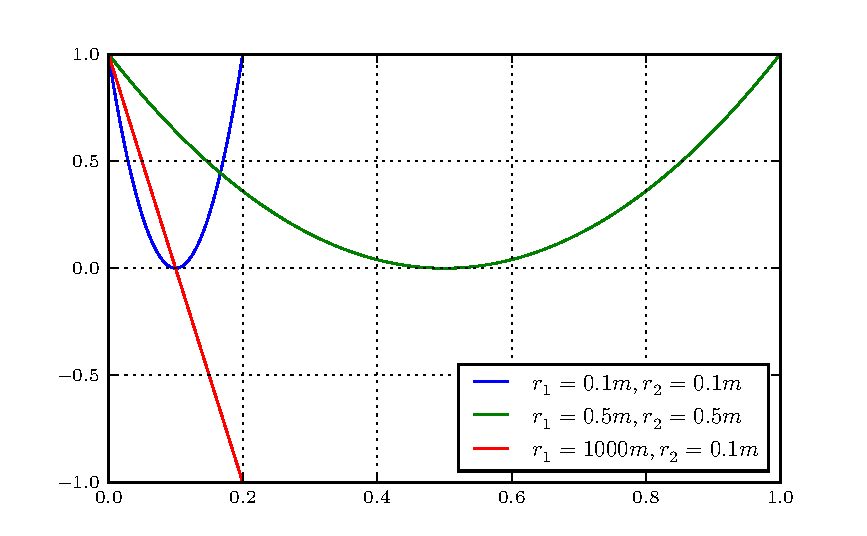
\includegraphics[height=6cm]{Stabilisationsparameter.pdf} 
  \caption{Stabilitätsbedingung des Resonators}
  \label{fig:stabi}
\end{figure}
Aus dem Diagramm kann abgelesen werden, dass bei Verwendung zweier Spiegel mit einem Krümmungsradius von 
\begin{equation}
  r_1 = 1400 \text{m}
  \label{eqn:rad1}
\end{equation}
die Maximal zu erwartenden Reichweite
\begin{equation}
  R_\text{1 max} = 2.8 \, \text{m}
  \label{eqn:rmax1}
\end{equation}
ist. In diesem Bereich läuft der Laser stabil und es kann ein Laserstrahl detektiert werden. Dies kann jedoch im Experiment nicht verifiziert werden, da die Schiene auf welche die Resonatorspiegel sitzen zu kurz ist. Bei der Verwedung von einem graden und einem Spiegel Krümmungsradiuses $r_1$ ergibt sich eine theoretische Reichweite von
\begin{equation}
  R_\text{2 max} = 1.4 \, \text{m} \ .
  \label{eqn:rmax2}
\end{equation}
Diese Reichweite wird verifiziert indem die Intensität der gemessenen Laserstrahlung von 100 \mu A bei einem Resonatorabstand von 140 auf 2 \mu A abfällt und der Laserstahl für weitere Reichweiten nicht weiter zu detektieren ist.

\subsection{TEM-Moden}
Da die Intensität der Laserstrahlung selbst nicht gemessen werden kann wird stattdessen ein Photostrom einer Diode gemessen. Dieser ist proportional zur Intensität. Auf die Ströme welche in Tabelle \ref{tab:tem} aufgetragen sind, wird in der weiteren Auswertung noch eingegangenen.
\begin{table}
  \centering
  \begin{tabular}{c|c c}
     \toprule
     	Abstand / mm & TEM 00 I / µA & TEM 10 I / µA \\
     \midrule
     0		& 0.058		& 0.041	\\
     1		& 0.112		& 0.078	\\
     2		& 0.199		& 0.142	\\
     3		& 0.332		& 0.166	\\
     4		& 0.458		& 0.204	\\
     5		& 0.623		& 0.298	\\
     6		& 1.187		& 0.367	\\
     7		& 1.221		& 0.286	\\
     8		& 2.120		& 0.384	\\
     9		& 2.332		& 0.233	\\
     10		& 3.140		& 0.220	\\
     11		& 3.165		& 0.076	\\
     12		& 3.954		& 0.048	\\
     13		& 4.195		& 0.010	\\
     14		& 4.222		& 0.024	\\
     15		& 4.408		& 0.100	\\
     16		& 5.006		& 0.204	\\
     17		& 4.207		& 0.387	\\
     18		& 3.644		& 0.502	\\
     19		& 2.903		& 0.562	\\
     20		& 2.323		& 0.601	\\
     21		& 1.580		& 0.499	\\
     22		& 1.352		& 0.760	\\
     23		& 1.172		& 0.701	\\
     24		& 0.904		& 0.603	\\
     25		& 0.673		& 0.512	\\
     26		& 0.522		& 0.422	\\
     27		& 0.220		& 0.244	\\
     28		& 0.186		& 0.249	\\
     29		& 0.143		& 0.200	\\
     30		& 0.062		& 0.070	\\
     31		& 0.053		& 0.059	\\
     \bottomrule
  \end{tabular}
  \caption{Diodenstrom in Abhängigkeit des Abstandes}
  \label{tab:tem}
\end{table}
Im folgenden wird geprüft ob die Intensitäten entsprechend von den Hermitpolynomen bzw Laguerre-Polynomen abhängig sind.
\subsubsection{TEM$_\text{00}$-Mode}
Die niedrigste Mode, welche gleichzeitigt die höchste Intensität aufweist wird ohne eine Modenblede erzeugt. Die mittels Photodiode gemessenen Ströme der $TEM_{00}$ - Mode sind in Tabelle \ref{tab:tem} aufgeführt und in Abbildung \ref{fig:TEM00} abgebildet. Dabei wurde die Auslenkung der Diode gegen den Photostrom aufgetragen.
\begin{figure}
  \centering
  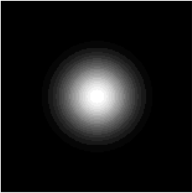
\includegraphics[height=6cm]{TEM00.pdf}
  \caption{Diodenstrom der Erste Mode in Abhängigkeit der Auslenkung der Diode}
  \label{fig:TEM00}
\end{figure}

Anhand von diesem wird entsprechend der Formel \ref{eqn:} ein Fit der Form 
\begin{equation}
  I_0 \cdot e^{- \frac{(x-\bar{x})^2}{\omega^2} }
  \label{eqn:gausian}
\end{equation}
wobei $I_0$ die Amplitude, $\bar{x}$ der Mittelwert und $\omega$ die die Standardabweichung der Gaußfunktion durch die Messwerte gelegt. Dieser Dient zum Vergleich mit dem Theoriewert und der Überprüfung ob die Intensitäten von den Laguerre-Polynomen abhängig sind. Es ergeben sich Fitparameter von 
\begin{eqnarray}
  a =& (\num{4.53 +- 0.08})	\\
  \bar{x} =& (\num{9.9 +- 0.2})	\\
  \omega =& (\num{-14.6 +-0.1})	
  \label{eqn:coef}
\end{eqnarray}
\subsubsection{TEM$_\text{10}$-Mode}
Zum erzeugen der ersten Mode wird ein Wolframdraht als Modenblende in den Strahlengang gestellt und solange ausjustiert bis der Strahlengang sich in zwei Punkte aufspaltet. Die mittels der Photodiode gemessenen Ströme in Abhängikeit der Auslenkung sind in Tabelle \ref{eqn:TEM} aufgetragen und in Abbildung \ref{fig:TEM10} dargestellt.
\begin{figure}
  \centering
  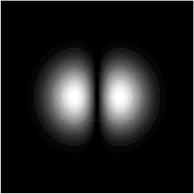
\includegraphics[height=6cm]{TEM10.pdf}
  \caption{Diodenstrom der Erste Mode in Abhängigkeit der Auslenkung der Diode}
  \label{fig:TEM10}
\end{figure}
Das zweite Hermitpolynom lautet
\begin{equation}
  H_q^p = 4x^2 - 2
  \label{eqn:Herm}
\end{equation}
Daraus ergibt sich der Fit der Form 
\begin{equation}
  I_0 \cdot 8 \frac{\left( x - \bar{x} \right)}{\omega^2} \cdot e^{-2 \frac{\left( x - \bar{x} \right)^2}{\omega^2}}
  \label{eqn:TEM10}
\end{equation}
welcher durch die Messwerte gelegt wird um, diese mit den Theoretischen Vorhersage zu vergleichen. Die Fitparameter sind
\begin{eqnarray}
  I_0 =& \num{0.36 +- 0.03}	\\
  \bar{x} =& \num{10.0 +- 0.5} \\
  \omega =& \num{14.1 +- 0.4}
\end{eqnarray}

\subsection{Polarisation der Laserstrahlung}

\begin{figure}
  \centering
  \includegraphics[height=6cm]{Polar.pdf}
  \caption{<+caption text+>}
  \label{fig:}
\end{figure}
\subsection{Wellenlänge des Lasers}
Zur bestimmung der Wellenlänge des Lasers wird ein Gitter der Gitterkonstanten 
\begin{equation}
  G = 10^5 \, \frac{1}{\text{m}}
  \label{eqn:constg}
\end{equation}
in den Laserstrahl gestellt. Im Abstand 
\begin{equation}
  L = 1.741 \, \text{m}
  \label{eqn:K}
\end{equation}
wird vom Schirm der Abstand der einzelnen Nebenmaxima ausgemessen. Die Abstände $a$ der einzelen Nebenmaxima vom Hauptmaxima sind in Tabelle \ref{tab:max} aufgetragen.
\begin{table}
  \centering
  \begin{tabular}{c c c}
    \toprule
    n-tes Maxima & $a_\text{links}$ $\frac{1}{\text{cm}}$ & $a_\text{rechts}$ $\frac{1}{\text{cm}}$ \\
    \midrule
	1 & 11.2 & 11.0 \\
	2 & 22.5 & 22.2 \\
	3 & 34.3 & 33.8 \\
    \bottomrule
  \end{tabular}
  \caption{Abstand der Nebenmaxima vom Hauptmaxima}
  \label{tab:max}
\end{table}
Aus den Abständen lässt sich anhand von Formel \ref{eqn:lambda} die Wellenlänge des Lasers berechnen. Sie beträgt 
\begin{equation}
  \lambda = (\num{652 +- 8}) \, \text{nm} \ .
\end{equation}
